% These are the lecture notes for my CSCI360 course SPRING 2017
% at John Jay College of Criminal Justice. They are based largely on
% Schneier's Applied Cryptography.

% Feel free to edit these slides and use them for your own courses.
% HOWEVER DO NOT REMOVE THESE LINES!
% Email me at: awood [at] jjay.cuny.edu
% or at: awood [at] gradcenter.cuny.edu


\documentclass{beamer}

\usepackage{tikz}
\usetikzlibrary{calc}

\usepackage{forest}
\usepackage{verbatim}
\usepackage{color}
\usepackage{amsmath}
\usepackage{graphicx}
\usepackage{caption}



\setbeamertemplate{footline}[frame number]
\setbeamertemplate{navigation symbols}{} 

\newtheorem{thm}{Theorem}[section]
\newtheorem{lem}{Lemma}
\newtheorem{cl}{Claim}
\newtheorem{cor}{Corollary}[section]
\newtheorem{conj}{Conjecture}
\newtheorem{quest}{Question}
\newtheorem{defn}{Definition}[section]
\newtheorem{obs}{Observation}[section]
\newtheorem{exam}{Example}

\newcommand{\im}{\operatorname{im}}
\newcommand{\id}{\operatorname{id}}
\newcommand{\interior}{\operatorname{int}}
\newcommand{\bdry}{\operatorname{bdry}}
\newcommand{\<}{\langle}
\renewcommand{\>}{\rangle}
\newcommand{\Gab}{(G_\phi)^{ab}} 
\newcommand{\phibar}{\bar{\phi}}
\newcommand{\Z}{\mathbb{Z}}
\newcommand{\N}{\mathbb{N}}
\newcommand{\Q}{\mathbb{Q}}
\newcommand{\R}{\mathbb{R}}
\newcommand{\C}{\mathbb{C}}
\newcommand{\A}{\mathcal{A}}
\newcommand{\OO}{\mathcal{O}}
\newcommand{\UU}{\mathcal{U}}
\newcommand{\power}{2^{\{P_1, \cdots , P_n\}}}
\newcommand{\bp}{\begin{problem}}
\newcommand{\ep}{\end{problem}}
\newcommand{\ba}{\begin{answer}}
\newcommand{\ea}{\end{answer}}
\newcommand{\ds}{\displaystyle}
\newcommand{\ben}{\renewcommand{\theenumi}{\alph{enumi}}
\renewcommand{\labelenumi}{(\theenumi)}\begin{enumerate}}
\newcommand{\een}{\end{enumerate}}
\newcommand{\Hess}{\operatorname{Hessian}}
\newcommand{\Aut}{\mathrm{Aut}}
\newcommand{\Inn}{\mathrm{Inn}}
\newcommand{\Out}{\mathrm{Out}}
\newcommand{\End}{\mathrm{End}}


\mode<presentation>
{
%  \usetheme{default}
  \setbeamercovered{invisible}
}


\usepackage[english]{babel}
\usepackage[latin1]{inputenc}
\usepackage{times}
\usepackage[T1]{fontenc}
\usepackage{stmaryrd}

%\usetheme{default}
%\usetheme{AnnArbor}
%\usetheme{Antibes}
%\usetheme{Bergen}
%\usetheme{Berkeley}
%\usetheme{Berlin}
%\usetheme{Boadilla}
%\usetheme{CambridgeUS}
%\usetheme{Copenhagen}
%\usetheme{Darmstadt}
%\usetheme{Dresden}
%\usetheme{Frankfurt}
%\usetheme{Goettingen}
%\usetheme{Hannover}
%\usetheme{Ilmenau}
%\usetheme{JuanLesPins}
%\usetheme{Luebeck}
%\usetheme{Madrid}
%\usetheme{Malmoe}
%\usetheme{Marburg}
%\usetheme{Montpellier}
%\usetheme{PaloAlto}
%\usetheme{Pittsburgh}
%\usetheme{Rochester}
\usetheme{Singapore}
%\usetheme{Szeged}
%\usetheme{Warsaw}

%\usecolortheme{default}
%\usecolortheme{albatross}
\usecolortheme{beaver}
%\usecolortheme{beetle}
%\usecolortheme{crane}
%\usecolortheme{dolphin}
%\usecolortheme{dove} % grey, white, yellow
%\usecolortheme{fly} %grey, yellow
%\usecolortheme{lily} %white, yellow, blue
%\usecolortheme{orchid}
%\usecolortheme{rose}
%\usecolortheme{seagull}
%\usecolortheme{seahorse}
%\usecolortheme{whale}
%\usecolortheme{wolverine}

% Title page

\title[HF]{Hash Functions}

\subtitle{Based on \emph{Applied Cryptography} by Schneier, Chapter 18}

\author
{Lecture notes of Alexander Wood \\ \scriptsize \href{mailto:awood@jjay.cuny.edu}{awood@jjay.cuny.edu}}
\institute[JJay]{John Jay College of Criminal Justice}  

\date{}

\begin{document}

% Remove 'figure' text from figure captions 
\setbeamertemplate{caption}{\raggedright\insertcaption\par}

\begin{frame}
  \titlepage
\end{frame}


\begin{frame}
\frametitle{One-Way Hash Functions}

A \textbf{one-way hash function} $H(M)$ takes as input a message $M$ of arbitrary length. It returns a value $h$ of fixed length $m$ called a \textbf{hash value}.

\begin{figure}
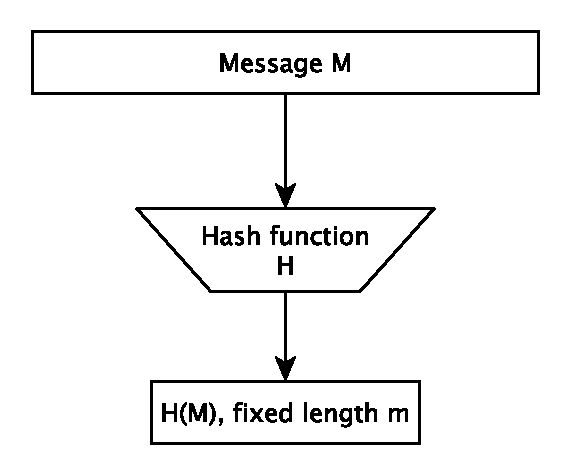
\includegraphics[scale=.6]{IMG/hash.pdf}
\end{figure}
\end{frame}

\begin{frame}
\frametitle{Hash Function Properties: Review}

Let $H$ be a one-way hash function and say $H(M) = h$. $H$ must satisfy the following properties:
\begin{itemize}
\item Given $M$ it is easy to compute $h$. In other words, $H(M)$ is a fast operation.
\item Given $h$, it is hard to compute $M$ such that $H(M) = h$.
\item Given $M$, it is hard to find another message $M'$ such that $H(M) = H(M')$.
\end{itemize}
\end{frame}


\begin{frame}
\frametitle{Collision-Resistance}

The property of \textbf{collision-resistance} states that it is hard to find \emph{any} two messages $M$ and $M'$ such that $H(M) = H(M')$. 
\end{frame}


\begin{frame}
\frametitle{Ideal Hash Functions}

The \textbf{ideal hash function} behaves like a random mapping from the set of possible input values to the set of possible output values.
\end{frame}


\begin{frame}
\frametitle{Attacks on Hash Functions}

An \textbf{attack on a hash function} is a non-generic method of distinguishing between the hash function and an ideal hash function.
\end{frame}


\begin{frame}
\frametitle{Designing Hash Functions}

How do we design a function which takes an input of \emph{arbitrary} length? Often we instead design a function which takes a value of a fixed size $m$ and outputs a value of a fixed length $n$. 
\begin{figure}
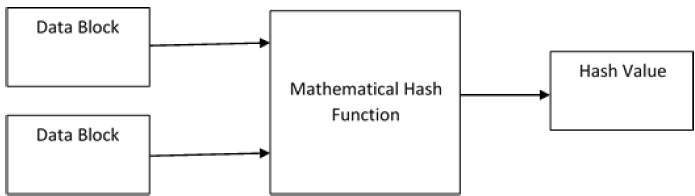
\includegraphics[scale=.6]{IMG/hash2}
\end{figure}
\end{frame}


\begin{frame}
\frametitle{Designing Hash Functions}

We hash a message by sectioning it into blocks of fixed size $m$, say $M_1,\dots, M_k$. Let $S$ be some \textbf{seed value} of size $m$. We compute as follows:
\begin{itemize}
\item $H_1 = H(S, M_1)$
\item $H_2 = H(H_1, M_2)$
\item $\cdots$
\item $H_k = H(H_{k-1}, M_k)$
\end{itemize}
where $H_k$ is the final output, or the hash value. 
\end{frame}

\begin{frame}
\frametitle{Sequential Applications of Hashing}

The following figure illustrates this concept. 
\begin{figure}
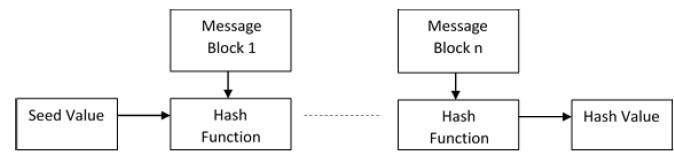
\includegraphics[scale=.5]{IMG/hash3}
\end{figure}

This is known as an \textbf{avalance effect}. The hash of the entire message is the hash of the last block.
\end{frame}




\begin{frame}
\frametitle{(Non-)Example 1}

First we look at an iterative hash function which is \emph{not} secure to illustrate what we do \emph{not} want. \newline

Refer to \emph{Cryptography Engineering} section 5.2.1 for more details on this non-example. 
\end{frame}


\begin{frame}[fragile]
\frametitle{(Non-)Example 1}

Let's build a hash function from AES (the Advanced Encryption Standard) with a $256$-bit key. 
\begin{enumerate}
\item Pad the message and break it into $128$-bit blocks $m_1, \dots, m_K$. 
\item Set $H_0:=$ \verb|00...0|, a $128$-bit block of all zeroes. 
\item Compute $H_i = \verb|AES|_K(H_{i-1}\oplus m_i)$ for $1\le i \le K$.
\item Output hash value $H_K$.
\end{enumerate}
\end{frame}


\begin{frame}
\frametitle{(Non-)Example 1}

\begin{figure}
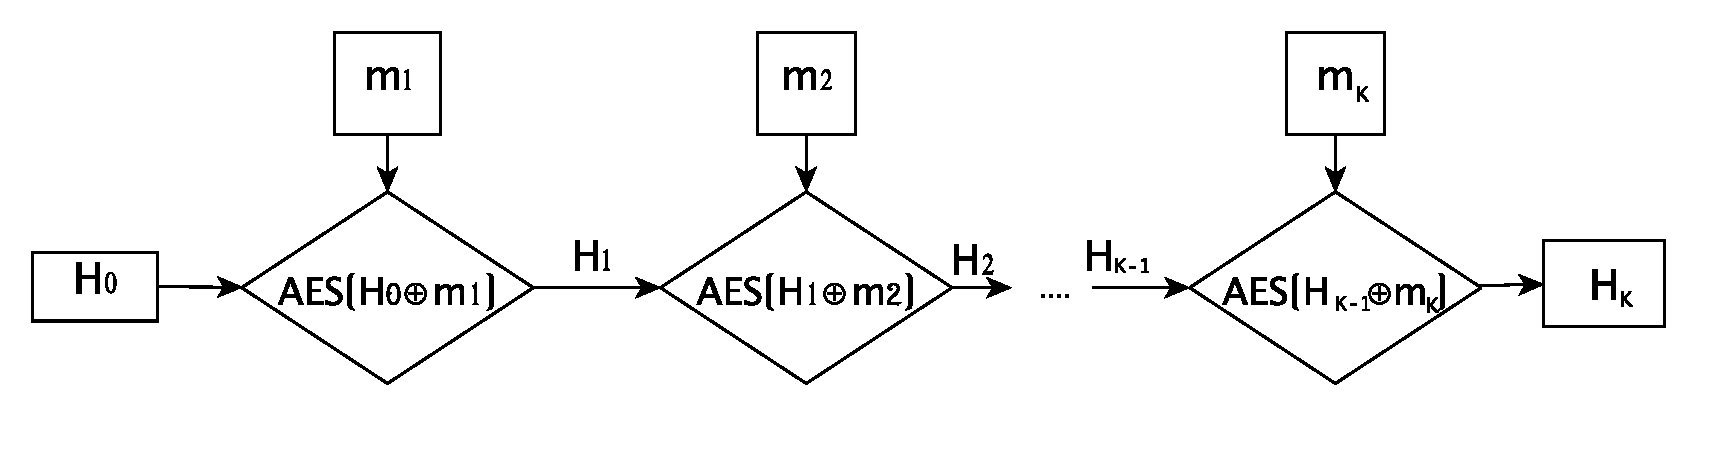
\includegraphics[scale=.4]{IMG/nonexample}
\end{figure}
\end{frame}


\begin{frame}
\frametitle{(Non-)Example 1: Attack}

Split a message $m$ into two blocks, $m_1$ and $m_2$. Let $m_1' = m_1 \oplus H_1$ and $m_2' = H_2\oplus m_2\oplus H_1$. Let $m' $ be the message that splits into $m_1'$ and $m_1'$ after hashing.\newline

What does $m'$ hash to?
\end{frame}

\begin{frame}
\frametitle{(Non-)Example 1: Attack}

\begin{figure}
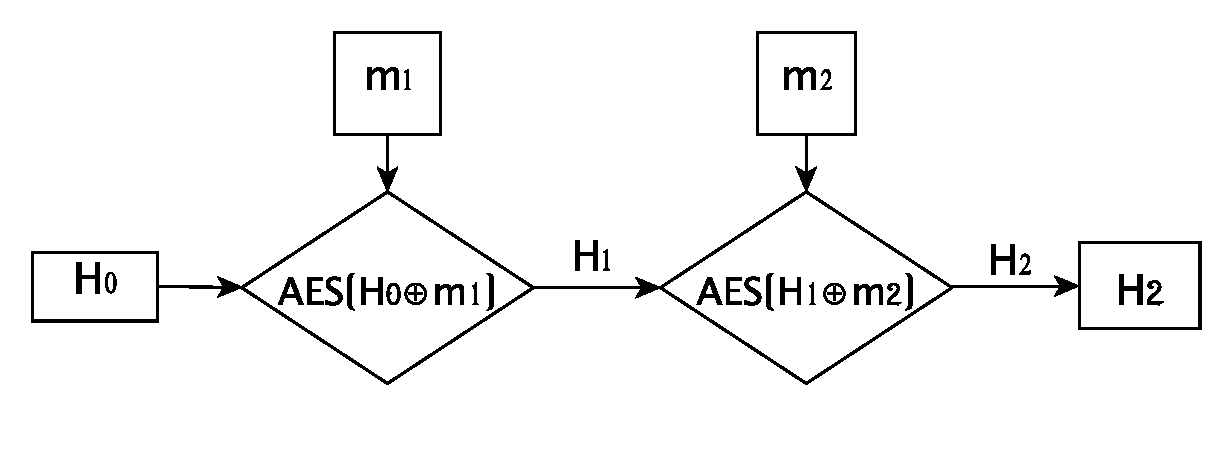
\includegraphics[scale=.5]{IMG/nonexample1}
\end{figure}

\begin{figure}
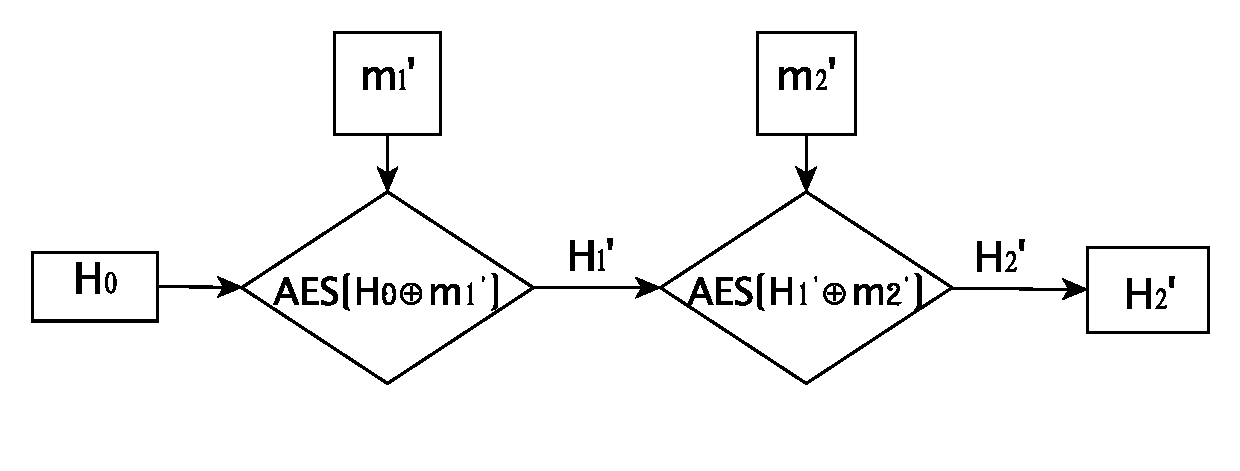
\includegraphics[scale=.5]{IMG/nonexample2}
\end{figure}
\end{frame}


\begin{frame}
\frametitle{(Non-)Example 1: Attack}

$m'$ hashes as follows:
\begin{enumerate}[1)]
\item $m_1' = m_1 \oplus H_1$, $m_2' = H_2\oplus m_2 \oplus H_1$
\item $H_1' = AES(H_0 \oplus m_1') = AES(H_0 \oplus H_1 \oplus m_1)$
\item Observe that:
\begin{align*}
H_2'& = AES(H_1' \oplus m_2')\\
	& = AES(AES(H_0 \oplus H_1 \oplus m_1)\oplus H_1\oplus H_2\oplus m_2)\\
	& = AES(H_2 \oplus H_1 \oplus H_2\oplus m_2)\\
	&= AES(H_1\oplus m_2) \\
	&= H_2
\end{align*}
\end{enumerate}
\textbf{We found a collision!}
\end{frame}


\begin{frame}
\frametitle{MD5}

The MD5 algorithm is one of the \textbf{Message Digest} functions designed by Ronald Rivest in 1991. It has $128$-bit output length and was thought for some time to be collision-resistant. \newline

In 2004 a group of Chinese cryptanalysts demonstrated a method for finding a collision. Now, collisions can be found in under one minute. 
\end{frame}


\begin{frame}
\frametitle{SHA-0}

The \textbf{Secure Hash Algorithm SHA-0}, designed by the NSA, is the first in a series of algorithms standardized by NIST. It was published in 1993. \newline

SHA-0 was withdrawn due to an unspecified weakness the NSA found within the algorithm. 
\end{frame}


\begin{frame}
\frametitle{SHA-1}

SHA-1 was the successor to SHA-0 in 1995. It has $160$-bit output. The birthday bound for this function is only $2^{80}$ steps; however, it was conjectured that a collision could be found in significantly fewer steps than this. \newline

This conjecture proved correct. Starting in 2005, various cryptologists published their own methods of attack which took well below $2^{80}$ steps. \newline

The first published collision was found this year, in February 2017! Google generated two different PDF files which have the same SHA-1 hash. It took them approximaetely $2^{63.1}$ evaluations. They called this the SHAttered attack.
\end{frame}

\begin{frame}
\frametitle{SHA-2}

SHA-2 was designed by the NSA and published in 2002. It is comprised of six related functions: SHA-SHA-224, SHA-256, SHA-384, SHA-512, SHA-512/224, SHA-512/256, which are 224, 256, 384 or 512 bits. \newline

The attacks against SHA-1 have not been successfuly extended to attack SHA-2. 
\end{frame}

\begin{frame}
\frametitle{SHA-3}

In 2007, NIST announced a competition to design a new cryptographic hash function. NIST selected the Keccack algorithm as the contest winner in 2012 and was standardized by NIST as SHA-3 in August 2015. 
\end{frame}

\begin{frame}
\frametitle{Video: Overview of SHA}

If interested you may watch the following overview of how SHA works, broadly:

\url{https://www.youtube.com/watch?v=5OVb4I5fhKI}
\end{frame}


\begin{frame}
\frametitle{Video: SHA-1}

If interested you may watch the following video of how SHA1 works:

\url{https://www.youtube.com/watch?v=aLvwpJcOy6s}
\end{frame}


\begin{frame}[fragile]
\frametitle{Python: hashlib}

We will learn how to implement Python's \verb|hashlib| module.\newline

\textbf{Please open IDLE on your computers so that we may all implement the following together.} \newline

The documentation as well as source code for \verb|hashlib| is available here:
\url{https://docs.python.org/3/library/hashlib.html}
\end{frame}


\begin{frame}[fragile]
\frametitle{Python: hashlib}

To use hashlib, type
\begin{verbatim}
>>> import hashlib
\end{verbatim}
into the active interpreter. 
\end{frame}



\begin{frame}[fragile]
\frametitle{Python: hashlib}

There is one constructor method named for each type of hash. All return a hash object with the same interface.\newline

To see what algorithms we can implement using \verb|hashlib|, type in the following command to your interpreter:
\begin{verbatim}
>>> hashlib.algorithms_guaranteed
\end{verbatim}
\end{frame}



\begin{frame}[fragile]
\frametitle{Python: hashlib}

Let's start with \verb|MD5|.  Enter the following commands, one-by-one.
\begin{verbatim}
md5object = hashlib.md5(b'Hello World')
print(hash_object.hexdigest())
\end{verbatim}

The \verb|b| which precedes the string literal converts the string to bytes.
\end{frame}


\begin{frame}[fragile]
\frametitle{Python: hashlib}

Now enter the following, one by one. 

\begin{verbatim}
>>> m = hashlib.md5()
>>> m.update(b"I know when that hotline bling")
>>> m.update(b" that can only mean one thing")
>>> m.digest()
>>> m.digest_size
>>> m.block_size
\end{verbatim}
\end{frame}


\begin{frame}[fragile]
\frametitle{Python: hashlib}

\begin{verbatim}
m = hashlib.md5()
\end{verbatim}

Create a md5 hash object. 
\end{frame}

\begin{frame}[fragile]
\frametitle{Python: hashlib}
\begin{verbatim}
>>> m.update(b"I know when that hotline bling")
>>> m.update(b" that can only mean one thing")
\end{verbatim}
The \verb|update| method updates the hash object with the argument in the parentheses. The input must be in byte format. It works by appending. For example, \verb|m.update(b'a')| followed by \verb|m.update(b'z')| is equivalent to \verb|m.update(b'az')|.
\end{frame}

\begin{frame}[fragile]
\frametitle{Python: hashlib}

\verb|m.digest()| returns the digest of the data passed to the \verb|update()| method so far. This is a bytes object of size \verb|digest_size| which may contain bytes in the whole range from 0 to 255.\newline

\verb|m.hexdigest()| is like \verb|digest()| except the digest is returned as a string object of double length, containing only hexadecimal digits. 
\end{frame}

\begin{frame}[fragile]
\frametitle{Python: hashlib}

\begin{verbatim}
>>> m.digest_size
>>> m.block_size
\end{verbatim}

Return the attributes \verb|digest_size| (size of resulting hash in bytes) and \verb|block_size| (size of internal block size in hashing algorithm).
\end{frame}

\begin{frame}
\frametitle{Python: hashlib}

Let's do the same as above with the remaining hash algorithms.
\end{frame}


\begin{frame}[fragile]
\frametitle{Python: hashlib, SHA-1}

 Enter the commands one-by-one in the active python interpreter. 
\begin{verbatim}
import hashlib
hash_object = hashlib.sha1(b'Hello World')
hex_dig = hash_object.hexdigest()
print(hex_dig)
blocksize = hash_object.block_size
digestsize = hash_object.digest_size
print(blocksize)
print(digestsize)
\end{verbatim}
\end{frame}



\begin{frame}[fragile]
\frametitle{Python: hashlib, SHA-224}
 Enter the commands one-by-one in the active python interpreter. 
\begin{verbatim}
import hashlib
hash_object = hashlib.sha224(b'Hello World')
hex_dig = hash_object.hexdigest()
print(hex_dig)
blocksize = hash_object.block_size
digestsize = hash_object.digest_size
print(blocksize)
print(digestsize)
\end{verbatim}
\end{frame}


\begin{frame}[fragile]
\frametitle{Python: hashlib, SHA-256}
 Enter the commands one-by-one in the active python interpreter. 
\begin{verbatim}
import hashlib
hash_object = hashlib.sha256(b'Hello World')
hex_dig = hash_object.hexdigest()
print(hex_dig)
blocksize = hash_object.block_size
digestsize = hash_object.digest_size
print(blocksize)
print(digestsize)
\end{verbatim}
\end{frame}

\begin{frame}[fragile]
\frametitle{Python: hashlib, SHA-384}
 Enter the commands one-by-one in the active python interpreter. 
\begin{verbatim}
import hashlib
hash_object = hashlib.sha384(b'Hello World')
hex_dig = hash_object.hexdigest()
print(hex_dig)
blocksize = hash_object.block_size
digestsize = hash_object.digest_size
print(blocksize)
print(digestsize)
\end{verbatim}
\end{frame}

\begin{frame}[fragile]
\frametitle{Python: hashlib, SHA-512}
 Enter the commands one-by-one in the active python interpreter. 
\begin{verbatim}
import hashlib
hash_object = hashlib.sha512(b'Hello World')
hex_dig = hash_object.hexdigest()
print(hex_dig)
blocksize = hash_object.block_size
digestsize = hash_object.digest_size
print(blocksize)
print(digestsize)
\end{verbatim}
\end{frame}


\begin{frame}
\frametitle{References}

\begin{itemize}
\item \emph{Applied Cryptography} By Schneier, Chapter 18
\item The HashLib documentation: \url{https://docs.python.org/3/library/hashlib.html}
\item Python implementations: \url{http://pythoncentral.io/hashing-strings-with-python/}
\end{itemize}
\end{frame}
\end{document}


